% This TeX document is part of the manual of the GNU Astronomy
% Utilities (Gnuastro). A Makefile is also distributed which allows
% you to compile this TeX file in the desired manner.
%
% Original author:
%     Mohammad Akhlaghi <mohammad@akhlaghi.org>
% Contributing author(s):
% Copyright (C) 2016-2018, Free Software Foundation, Inc.
%
% Gnuastro is free software: you can redistribute it and/or modify it
% under the terms of the GNU General Public License as published by
% the Free Software Foundation, either version 3 of the License, or
% (at your option) any later version.
%
% Gnuastro is distributed in the hope that it will be useful, but
% WITHOUT ANY WARRANTY; without even the implied warranty of
% MERCHANTABILITY or FITNESS FOR A PARTICULAR PURPOSE.  See the GNU
% General Public License for more details.
%
% You should have received a copy of the GNU General Public License
% along with Gnuastro. If not, see <http://www.gnu.org/licenses/>.

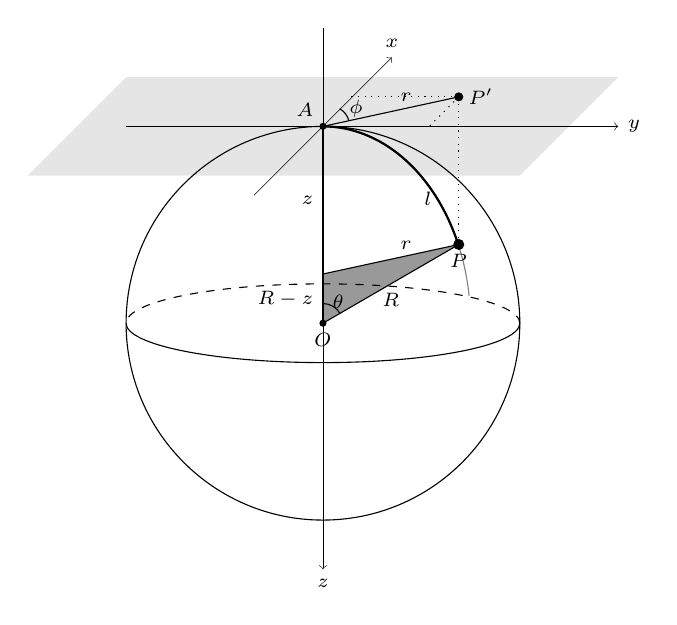
\begin{tikzpicture}[scale=1.25]
  \tikzstyle{every node}=[font=\scriptsize]
  %parallelogram: 2D surface
  \fill[fill=black!10!white]
  (-1.5,0.5) -- ++(5,0) -- ++(-1,-1) -- ++(-5,0) -- cycle;

  %Triangle:
  \filldraw[fill=black!40!white, draw=black]
  (0.5,-2) -- node[anchor=north]{$R$}(1.88,-1.2)
  -- node[anchor=south west]{$r$}(0.5, -1.5) -- cycle;
  \draw (0.5,-1.8) arc (90:30:0.2);
  \draw (0.5,0) -- node[anchor=east]{$z$}(0.5,-1.5)
  -- node[anchor=east]{$R-z$}(0.5,-2);
  \draw (0.5,-1.95) node[anchor=south west]{$\theta$};

  %Cartesian Coordinates, sphere and their names
  \draw[<-, very thin] (1.2,0.7) -- (-0.2,-0.7);
  \draw (1.2,0.7) node[anchor=south]{$x$};

  \draw[->, very thin] (-1.5,0) -- (3.5,0);
  \draw (3.5,0) node[anchor=west]{$y$};

  \draw[->, very thin] (0.5,1) -- (0.5,-4.5);
  \draw (0.5,-4.5) node[anchor=north]{$z$};

  \draw (0.5,-2) circle (2);
  \draw (-1.5,-2) arc (180:360:2 and 0.4);
  \draw[dashed] (2.5,-2) arc (0:180:2 and 0.4);

  \filldraw (0.5,0) circle (0.03);
  \draw (0.5,0) node[anchor=south east]{$A$};

  \filldraw (0.5,-2) circle (0.03);
  \draw (0.5,-2) node[anchor=north]{$O$};

  \draw (0.67,0.18) arc (60:15:0.2);
  \draw (0.67,0.18) node[anchor=west]{$\phi$};

  %P and it's arcs
  \draw[thin, gray] (0.5,0) arc(90:8:1.5 and 2);
  \draw[thick] (0.5,0) arc(90:25:1.5 and 2);

  \filldraw (1.88,-1.2) circle (0.05);
  \draw (1.88,-1.2) node[anchor=north]{$P$};
  \filldraw (1.88,0.3) circle (0.04);
  \draw[dotted] (1.88,-1.2) -- (1.88, 0.3);

  %Images of P and P' on 2D plane:
  \draw (1.88,0.3) node[anchor=west]{$P'$};
  \draw (0.5,0) -- node[anchor=south west]{$r$}(1.88, 0.3);
  \draw[dotted] (1.88,0.3) -- ++(-1.1,0);
  \draw[dotted] (1.88,0.3) -- ++(-0.3,-0.3);

  % Label chi:
  \draw (1.43, -0.9) node[anchor=south west]{$l$};
\end{tikzpicture}
